\chapter{Análisis (Datos, Arquitectura, Software, Algoritmos)}

Este capítulo cuenta cómo está armado BOLD5000, el preprocesamiento, los
pares (estímulo, beta), las particiones, el modelo entidad-relación, el prototipeo,
el diagrama UML del pipeline, una mirada a los algoritmos existentes y a los
propios, y los requerimientos del sistema

\section{Base de datos existente: BOLD5000}

\subsection{Descripción general}

BOLD5000~\cite{chang2019bold5000} junta a cuatro sujetos (CSI1–CSI4) que vieron 5254 imágenes
únicas sacadas de COCO, ImageNet y Scenes UnderStanding (SUN). Los
volúmenes están en OpenNeuro (ds001499) en formato BIDS, lo que hace
bastante más fácil bajarlos y preprocesarlos.

\subsection{Decisión: dataset existente vs.\ propio}

Armar un dataset propio quedó descartado desde el principio. Necesitaría
un escáner 3T, aprobación ética, más de 15 sesiones por sujeto y unos cincuenta
mil dólares de presupuesto. BOLD5000 alcanza en tamaño y calidad para
probar la hipótesis y encima es libre.

\section{Preprocesamiento}

\subsection{Descarga vía OpenNeuro CLI}

La descarga se queda solo con los betas preprocesados y las máscaras
corticales por sujeto. Así no se arrastran los volúmenes raw que no se usan:

\begin{lstlisting}[language=bash, caption=Descarga selectiva BOLD5000, label={lst:openneuro}]
openneuro download --snapshot 2.0.1 \
--include "derivatives/fmriprep/sub-*/ses-*/func/*_bold.nii.gz" \
--include "derivatives/spm/sub-*/sub-*_ROIs_TR34.mat" \
ds001499 ./data_bold5000/
\end{lstlisting}

\subsection{Máscara cortical visual}

Se usa la máscara cortical que viene con BOLD5000 (V1–V4 + LOC + PPA),
que deja cada volumen reducido a un vector de unos 5000 a 7000 vóxeles activos
por sujeto.

\subsection{Pares (estímulo, beta) y normalización}

Cada trial se empareja con la imagen que toca en \texttt{stimuli/}. Los betas se centran y 
se normalizan por sesión (z-score) para que la deriva de baseline no haga ruido.

\section{Análisis estadístico de la base de datos}

\subsection{Estadísticas descriptivas por sujeto}

\begin{table}[H]
\centering
\resizebox{\textwidth}{!}{
\begin{tabular}{| l | c | c | c | c | c |}
\hline
\textbf{Sujeto} & \textbf{Trials} & \textbf{Vóxeles} & \textbf{$\mu_\beta$} & \textbf{$\sigma_\beta$} & \textbf{Sesiones} \\ \hline
CSI1 & TBD & TBD & TBD & TBD & 15 \\ \hline
CSI2 & TBD & TBD & TBD & TBD & 15 \\ \hline
CSI3 & TBD & TBD & TBD & TBD & 15 \\ \hline
CSI4 & TBD & TBD & TBD & TBD & 9 \\ \hline
\end{tabular}
}
\caption[Estadísticas BOLD5000 por sujeto]{Conteo de trials, vóxeles activos en máscara visual, media y desviación de $\beta$, y sesiones por sujeto.}
\label{table:bold5000_stats}
\end{table}

\subsection{Matriz de correlación inter-vóxel}

Al observar las correlaciones entre pares de vóxeles dentro de la máscara visual afloran clusters funcionales (V1 frente a LOC), que son los que sostienen la partición jerárquica. Completaré la figura tras la corrida final.

\section{Modelo Entidad-Relación}

\begin{table}[H]
\centering
\begin{tabular}{| l | l |}
\hline
\textbf{Entidad} & \textbf{Atributos} \\ \hline
Sujeto       & subject\_id (PK), género, edad, n\_sesiones \\ \hline
Sesión       & session\_id (PK), subject\_id (FK), fecha, n\_trials \\ \hline
Trial        & trial\_id (PK), session\_id (FK), stim\_id (FK), TR\_offset \\ \hline
Estímulo     & stim\_id (PK), categoría (COCO/ImageNet/SUN), path \\ \hline
Beta         & trial\_id (FK), voxel\_idx, valor\_$\beta$ \\ \hline
Embedding    & stim\_id (FK), modelo (ViT-L/14), vector[768] \\ \hline
\end{tabular}
\caption[ER del dataset]{Modelo entidad-relación de pares (estímulo, beta, embedding).}
\label{table:er_dataset}
\end{table}

\section{Prototipeo y arquitectura}

\subsection{Diagrama de arquitectura}

La Figura~\ref{fig:arquitectura_pipeline} condensa el flujo en tres fases. El preprocesamiento arranca en \texttt{config.py} y lanza dos módulos en paralelo: \texttt{bold5000\_loader.py}, que construye las matrices $X$ de vóxeles por sujeto, y \texttt{extract\_vit\_features.py}, que obtiene los vectores $Y$ de embeddings CLIP ViT-L/14. El puente neuronal ajusta el Ridge Lineal con \texttt{train\_adapter.py} y \texttt{adapter\_ridge.py}; para el Ridge Estocástico basta con sumar el módulo \texttt{adapter\_ridge\_stoch.py}. Ya en inferencia, llega un fMRI de prueba, el adapter elegido lo proyecta a $\mathbb{R}^{768}$, \texttt{sd\_decoder.py} genera la reconstrucción y \texttt{visual\_evaluator.py} guarda el resultado.

\begin{figure}[H]
\centering
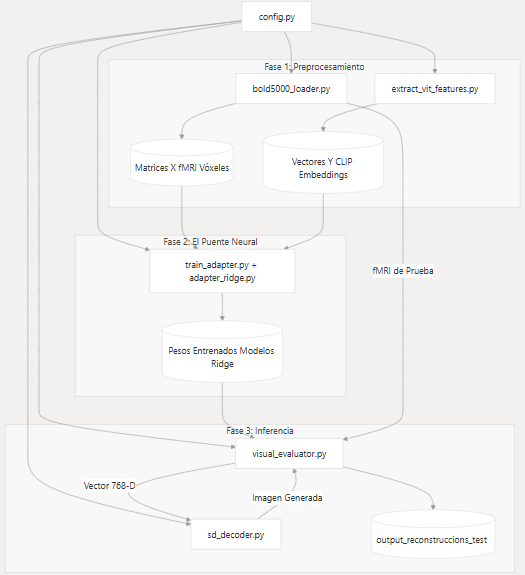
\includegraphics[width=0.85\textwidth]{Figures/arquitectura_pipeline.png}
\caption[Arquitectura del pipeline]{Arquitectura modular del sistema fMRI$\rightarrow$imagen. Tres fases secuenciales: preprocesamiento, puente neuronal (Ridge Lineal o Ridge Estocástico) y síntesis condicional con Stable Diffusion 2.1 unCLIP.}
\label{fig:arquitectura_pipeline}
\end{figure}

\section{Análisis de algoritmos existentes}

\subsection{Ridge regression cerrado}

Quien manda en el costo es el término $V^{3} + V^{2}N$, que viene de invertir $(\mathbf{X}^{\top}\mathbf{X} + \lambda\mathbf{I})^{-1}$. Con $V \approx 6000$ y $N \approx 4000$ el cálculo en CPU termina en menos de cinco minutos; si añado validación cruzada de 5 folds, ese tiempo se multiplica por cinco.

\subsection{Optimización SGLD del baseline VQGAN}

El baseline histórico VQGAN+VGG~\cite{koidemajima2024} pide 500 iteraciones por imagen, y cada una hace forward y backward sobre VGG, CLIP y VQGAN. En una RTX~3070 son entre 15 y 20 minutos por imagen, que bajan a 8--12 al meter bf16, TF32 y cacheo. No tomo esta ruta; solo la traigo como referencia.

\section{Análisis de algoritmos propios}

\subsection{Adapter Ridge Lineal}

Solución cerrada de la ecuación normal regularizada. Al lado del resto del pipeline, su costo es casi nulo (segundos en CPU). Es el predictor base y, a la vez, la referencia diagnóstica de todo el trabajo.

\subsection{Adapter Ridge Estocástico}

El predictor estocástico arranca del mapeo lineal y le monta encima una perturbación Gaussiana isotrópica:
\begin{equation}
\hat{\mathbf{e}}_{\mathrm{stoch}} = \mathbf{X}\hat{\boldsymbol{\beta}}_{\mathrm{Ridge}} + \sigma\,\boldsymbol{\xi}, \qquad \boldsymbol{\xi}\sim\mathcal{N}(\mathbf{0},\mathbf{I}_{D}).
\end{equation}
\myequations{Predictor Ridge Estocástico}
Antes de mandarlo al pipeline, renormalizo el embedding sobre la hiperesfera unidad. El $\sigma$ lo calibro en validación buscando la mayor pairwise accuracy sobre embeddings CLIP. La idea sale tal cual de MindEye y MindEye2~\cite{scotti2023mindeye,scotti2024mindeye2}, donde queda claro que llevar la predicción a zonas más densas del manifold CLIP mejora la respuesta del decodificador. Y lo logro sin entrenar un MLP residual entero: el costo sigue siendo el del Ridge más una transformación fija por trial.

\subsection{Selección de vóxeles: 3-Partition vs.\ partición biológica}

Elegir el mejor subconjunto de $k$ vóxeles dentro de un universo de $V \sim 60{,}000$ es, de por sí, un problema combinatorio. Si además exijo balanceo entre regiones funcionales, la tarea se reduce al clásico 3-Partition, NP-completo en sentido fuerte~\cite{garey1979computers} (la formalización está en el Cap.~2 \S2.4). Cuando la utilidad es submodular monótona, el greedy asegura una aproximación $1-1/e$~\cite{nemhauser1978,krause2014submodular}. Yo esquivo el problema apoyándome en la partición biológica que BOLD5000 ya trae (V1--V4, LOC, PPA): dejo la decisión combinatoria en manos de la biología y reservo al adapter la extracción de la información discriminativa.

\section{Requerimientos del sistema}

\subsection{Funcionales}

\begin{itemize}
\item[•] RF1: Leer los betas en formato HDF5 por sujeto y sesión.
\item[•] RF2: Ajustar el adapter Ridge Lineal mediante validación cruzada y, a partir de él, obtener el Ridge Estocástico calibrando $\sigma$.
\item[•] RF3: Inferir un embedding de 768 dimensiones a partir de un vector de vóxeles.
\item[•] RF4: Generar la reconstrucción con SD~2.1 unCLIP usando el embedding predicho.
\item[•] RF5: Calcular las seis métricas y exportarlas a CSV y HTML.
\end{itemize}

\subsection{No funcionales}

\begin{itemize}
\item[•] RNF1: Inferencia por debajo de diez segundos por trial en RTX~4070.
\item[•] RNF2: Pico de VRAM que no pase los 8~GB en bf16 con xformers.
\item[•] RNF3: Reproducibilidad bit a bit con seed fijo (42).
\item[•] RNF4: Código compatible con Python 3.12 y PyTorch 2.x.
\end{itemize}

\section{Particiones train/val/test}

\begin{table}[H]
\centering
\begin{tabular}{| l | c | c | c |}
\hline
\textbf{Sujeto} & \textbf{Train} & \textbf{Val} & \textbf{Test} \\ \hline
CSI1 & TBD & TBD & TBD \\ \hline
CSI2 & TBD & TBD & TBD \\ \hline
CSI3 & TBD & TBD & TBD \\ \hline
CSI4 & TBD & TBD & TBD \\ \hline
\end{tabular}
\caption[Particiones BOLD5000]{Pares (estímulo, beta) por sujeto y partición. Split por estímulo, no por trial, para evitar fuga.}
\label{table:bold5000_splits}
\end{table}

\afterpage{\blankpage}
